\section{Integer basins and a cosine continuation}
\label{sec:geometry}

For $(1,0,-1)$, integer capture means eventual entry into a phased
cycle. For its cosine continuation, a complex start belongs to the basin
if its iterates converge to the cycle at matching phases.

\subsection{Integer cycles and the phase-zero return}

Fix $d=(1,0,-1)$ and let
\[
 \Phi(n,i)=(T(n)+d_i,i+1\bmod3),\qquad
 F(n)=F_{d,0}^{(3)}(n).
\]
The safe integer state space consists of $n\ge0$ at phase zero and
$n\ge1$ at phases one and two. The following cycles are different
closed paths in that space.

\begin{proposition}[Exact nonnegative cycles]
\label{prop:geometry-cycles}
The augmented map has the cycles
\begin{align*}
 \Gamma_3:\quad &(0,0)\to(1,1)\to(2,2)\to(0,0),\\
 \Gamma_9:\quad &(1,0)\to(3,1)\to(5,2)\to(7,0)
 \to(12,1)\to(6,2)\\
 &\hspace{33mm}\to(2,0)\to(2,1)\to(1,2)\to(1,0).
\end{align*}
Their least augmented and scalar periods are respectively three and
nine. At phase zero, the first is the fixed point $F(0)=0$ and the
second is the three-cycle $1\mapsto7\mapsto2\mapsto1$.
\end{proposition}
\begin{proof}
Substitution in the signed shortcut rule verifies every arrow, including
$T(0)+1=1$ and $T(2)-1=0$. Within either displayed loop the augmented
states are distinct, so the first repeated augmented state occurs at
the stated length. The forcing is primitive of period three. The
period relation proved in Section~\ref{sec:foundations} shows that a
scalar cycle must already have period divisible by three. The three
different phase-zero values on $\Gamma_9$ rule out scalar period three.
\end{proof}

\begin{figure}[htbp]
 \centering
 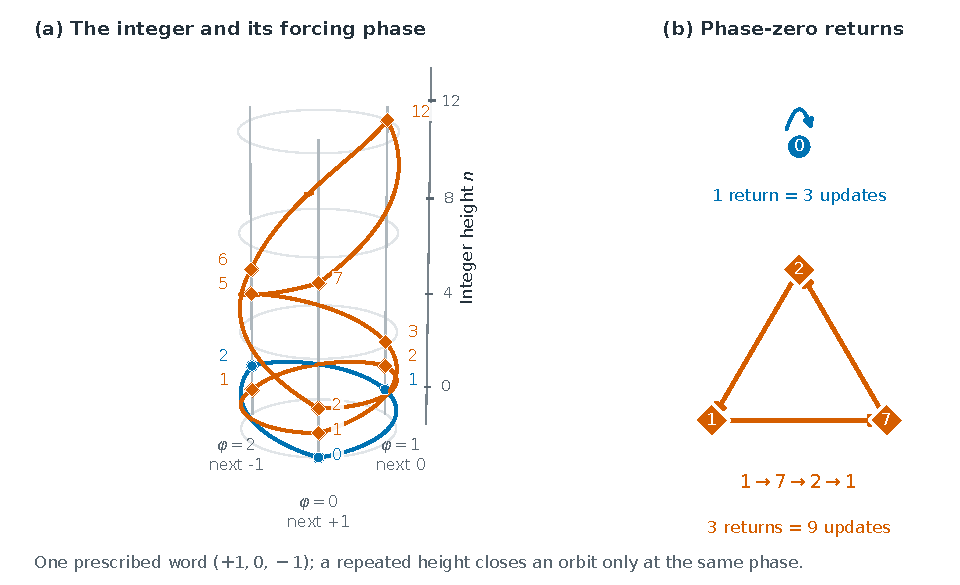
\includegraphics[width=.94\linewidth]{figures/phase_cycles.pdf}
 \caption{Exact integer cycles with the forcing phase retained. Sampling
 once every three physical updates gives a fixed point and a three-cycle
 of the phase-zero return. Equal scalar heights on different phase
 sheets are distinct states.}
 \label{fig:phase-cycles}
\end{figure}

At phase zero the eight return branches of Section~\ref{sec:inverse}
are, for $q\ge0$,

\begin{equation}\label{eq:geometry-return-table}
 F(8q+r)=3^{o_r}q+c_r,
 \qquad
 \begin{array}{c|rrrrrrrr}
 r&0&1&2&3&4&5&6&7\\\hline
 o_r&1&3&1&2&2&2&0&1\\
 c_r&0&7&1&4&7&6&0&2
 \end{array}
\end{equation}
At each of the three updates the coefficient of $q$ is even, so the
constant term fixes the parity on the entire ray.
\path{certificates/geometry/discrete.py} propagates both coefficients
and checks the cycles.

\begin{figure}[htbp]
 \centering
 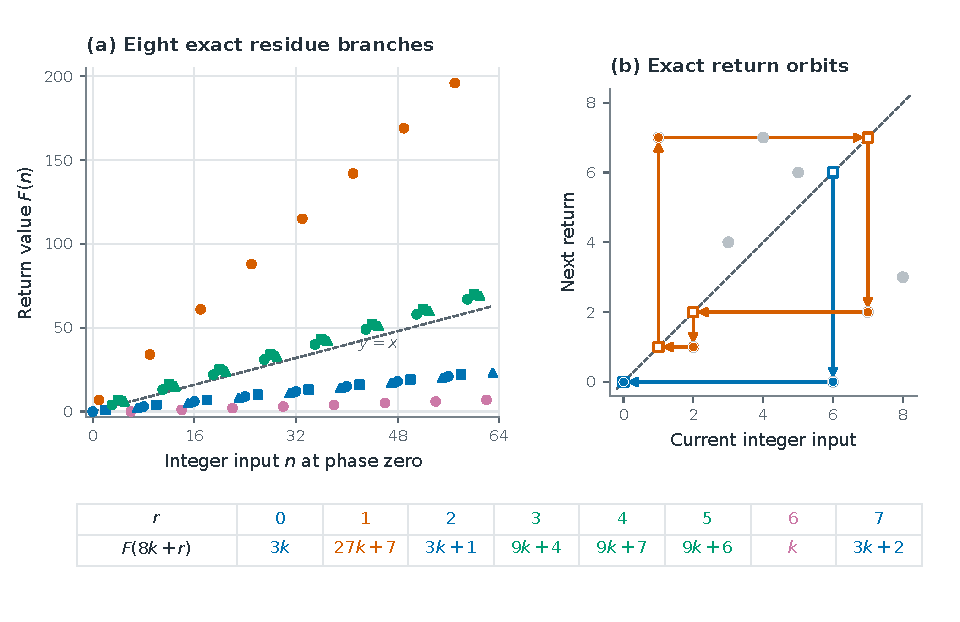
\includegraphics[width=.94\linewidth]{figures/integer_return.pdf}
 \caption{The eight residue-affine branches of the integer return and
 an exact return orbit. An affine branch applies only to its indicated
 residue class; a connecting line is a plotting aid, not a new
 continuous definition of the integer map.}
 \label{fig:integer-return}
\end{figure}

Let $\mathcal B_{3,i}$ and $\mathcal B_{9,i}$ denote the safe integer
seeds at phase $i$ eventually entering $\Gamma_3$ and $\Gamma_9$.
The basins are disjoint by determinism. Other cycles and unbounded safe
orbits remain possible.

\subsection{Basin interlacing and binary zooms}

\begin{corollary}[Both basins in every arithmetic neighborhood]
\label{cor:geometry-interlacing}
For every launch phase $i$, modulus $M\ge1$, and residue $a\bmod M$,
both $\mathcal B_{3,i}$ and $\mathcal B_{9,i}$ contain at least
$cX^\delta$ positive seeds at most $X$ in that residue class, for all
sufficiently large $X$. The positive constant and threshold may differ
between the two basins and may depend on the phase and progression;
$\delta$ is the exponent in Theorem~\ref{thm:inverse-growth}.
\end{corollary}
\begin{proof}
Apply Theorem~\ref{thm:inverse-growth} first to the safe augmented
target $(0,0)$ and then to $(1,0)$, with the prescribed launch phase
and progression. A predecessor of the first target belongs to
$\mathcal B_{3,i}$; a predecessor of the second belongs to
$\mathcal B_{9,i}$. The targets lie on the distinct cycles just proved.
\end{proof}

In particular, no finite number of low binary digits determines the
basin. By Proposition~\ref{prop:affine-parity}, a specified finite
input-parity word at a fixed phase is one residue class modulo a power
of two. The corollary gives arbitrarily large seeds in \emph{both}
basins with that same parity prefix. Even prescribing additional
ternary digits or any other fixed modulus does not change this fact.
For example, $9$ and $25$ are both $9\bmod16$, but their phase-zero
return orbits reach different cycles. The first follows
\[
 9\to34\to13\to15\to5\to6\to0,
\]
whereas the second eventually reaches $1\to7\to2\to1$.
The atlas interleaves the binary digits of each seed into two screen
coordinates. Each successive quadrant fixes two more low bits. A seed
receives a basin color when its integer trajectory reaches the cycle.
The remaining seeds stay unclassified at the iteration limit.

\begin{figure}[htbp]
 \centering
 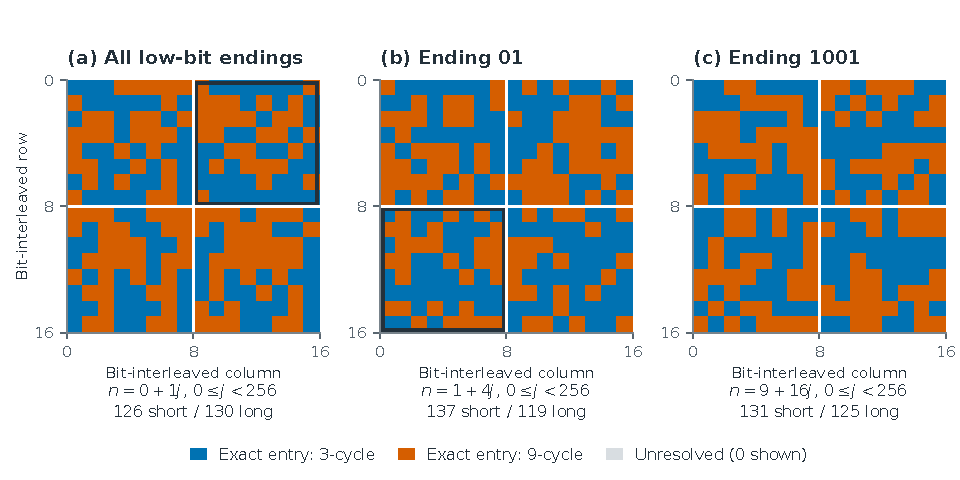
\includegraphics[width=.94\linewidth]{figures/binary_basins.pdf}
 \caption{An integer basin atlas arranged by low binary digits.
 Each colored sample is a particular integer with a replayed cycle
 destination. Corollary~\ref{cor:geometry-interlacing}, rather than the
 pixel count, proves that both basins occur in every fixed binary
 residue class at arbitrarily large heights.}
 \label{fig:binary-basins}
\end{figure}

One nested family of tiles is an \emph{exact copy} of the entire
integer dynamics, including any behavior that has not been classified.

\begin{proposition}[Exact binary zoom]\label{prop:binary-zoom}
Put $E(y)=8y+6$ and
$c_k=6(8^k-1)/7$. For every $k\ge0$ and $y\ge0$,
\begin{equation}\label{eq:binary-zoom}
 E^k(y)=8^ky+c_k,\qquad F^k(E^k(y))=y.
\end{equation}
Every nonnegative integer congruent to $c_k\pmod{8^k}$ has this
form with a unique $y\ge0$. Its first $3k$ physical input parities
are even. In particular, it belongs to a cycle basin at phase zero
if and only if its quotient seed $y$ belongs to that basin.
\end{proposition}
\begin{proof}
One literal lap is
\[
 8y+6\ \longmapsto\ 4y+4\ \longmapsto\ 2y+2
 \ \longmapsto\ y.
\]
All three input values are even, and the final value is at the initial
phase. Iteration proves the return and parity assertions. The affine
formula follows either by induction or by summing a geometric series.
Since $0\le c_k<8^k$, division with remainder proves the assertion
about every nonnegative member of the residue class. Appending a
finite initial path to a trajectory changes neither its eventual
cycle nor its failure to enter a specified cycle.
\end{proof}

Appending the three low bits $110$ is precisely the operation $E$.
For instance, $E^3(0)=438$ and $E^3(1)=950$ share nine low bits and
nine even inputs before reaching different cycles.
The all-depth identity is also certified by
\path{lean/inverse/Collatz/BinaryZoom.lean}; the figure is only a finite
view of that identity.

In the $2$-adic metric $|u-v|_2=2^{-v_2(u-v)}$, the two basins are
dense in the space of $2$-adic integers: each residue neighborhood
contains members of each basin by Corollary~\ref{cor:geometry-interlacing}.
The zoom identity gives the concrete common accumulation point
\[
 E^k(y)+\frac67=8^k\left(y+\frac67\right),
 \qquad E^k(y)\longrightarrow-\frac67\quad\text{in }\mathbb Z_2.
\]
For fixed $y\ge0$, these seeds tend to $+\infty$ in the real metric.
Membership in either basin fails to be ultimately periodic because
every residue class of any proposed period contains arbitrarily large
seeds from both basins. Their natural densities remain undetermined.

\subsection{The cosine continuation}

Between integer inputs we use the entire function

\begin{equation}\label{eq:cosine-extension}
 C(w)=w+\frac14-\left(\frac w2+\frac14\right)\cos(\pi w),
 \qquad w\in\mathbb C.
\end{equation}
On the real line this is Chamberland's interpolation
\cite{chamberland-1996,chamberland-survey}. At integers,
$\cos(\pi n)=(-1)^n$ gives $C(n)=T(n)$. The phased update is
$\Phi_C(w,i)=(C(w)+d_i,i+1\bmod3)$, with phase-zero return

\begin{equation}\label{eq:complex-return}
 R(w)=C\bigl(C(C(w)+1)\bigr)-1.
\end{equation}
Thus $R(n)=F(n)$ at every integer.

This interpolation is part of the model. For example,
$C(w)+\lambda\sin^2(\pi w)$ has the same values and first derivatives
at every integer for every fixed $\lambda$, while its values away from
the integers are different. Thus even exact knowledge of all integer
orbits and their linear multipliers does not specify the off-integer
function. Results about the following disks and separator refer to
\eqref{eq:cosine-extension} with the stated forcing.

Dumont and Reiter compare this cosine interpolation with a distinct
\emph{3-power} extension that agrees at integers and has the same
integer derivatives, while differing between the integers
\cite[Sections~1--2]{dumont-reiter-2003}.
Letherman, Schleicher and Wood construct selected entire extensions
for which all integers belong to the Fatou set and a noneventually
periodic integer would belong to a wandering domain
\cite{letherman-schleicher-wood-1999}.
Their family does not contain the cosine interpolation, as noted
explicitly by Dumont and Reiter \cite[Section~1]{dumont-reiter-2003}.
Those global Fatou-set conclusions therefore do not follow for $R$
from agreement with integer Collatz values.

The derivatives needed below are
\begin{align}
 C'(w)&=1-\tfrac12\cos(\pi w)
       +\pi(w/2+1/4)\sin(\pi w),\label{eq:cosine-derivative}\\
 C''(w)&=\pi\sin(\pi w)+\pi^2(w/2+1/4)\cos(\pi w).
 \label{eq:cosine-second}
\end{align}
In particular, $C'(n)=1/2$ at even integers and $3/2$ at odd
integers. An impulse is a translation, so it contributes derivative
one. A cycle with $L$ physical updates and $o$ odd integer inputs
therefore has multiplier $3^o/2^L$ over a \emph{complete} cycle.
For $\Gamma_3$ this is $3/8$; for $\Gamma_9$ it is $243/512$.
The one-lap derivative at the phase-zero point $1$ of $\Gamma_9$
is instead $27/8>1$. The following two laps have derivatives $3/8$
and $3/8$, and their product gives the contracting nine-step
multiplier. A growing portion of a return cycle is compatible with
attraction of the whole cycle.

\begin{proposition}[Attraction of admissible integer cycles]
\label{prop:integer-cycle-attraction}
Every nonnegative integer cycle of a nonzero conservative admissible
word is locally attracting under the phasewise cosine interpolation.
\end{proposition}
\begin{proof}
Every nonnegative periodic orbit lies in the safe domain: zero at a
height-one phase would remain zero until the next negative impulse
and then become negative. Use the binary height from
Proposition~\ref{prop:height-conjugacy} and write
$z_j=n_j+1-h_j>0$ along the cycle. Let
$e_j=n_j\bmod2$ and $\epsilon_j=z_j\bmod2$. The two height cases give
the same exact identity
\[
 2z_{j+1}=3^{e_j}z_j+\epsilon_j.
\]
Divide by $z_j$ and multiply around the cycle. If its length is $L$
and $o=\sum e_j$, then
\[
 2^L=\prod_{j=0}^{L-1}
       \left(3^{e_j}+\frac{\epsilon_j}{z_j}\right)
 \ge3^o.
\]
Equality is impossible because $L\ge1$ and powers of two and three
are different. Hence $3^o/2^L<1$. By the chain rule this is the
derivative of the full complex return at the periodic point. Continuity
of that derivative gives a small closed disk on which its modulus is
uniformly below one. Since the center is fixed, integration on line
segments makes that return a contraction mapping the disk into itself.
All points in the disk converge to the periodic point; the intermediate
phase maps give convergence along the entire cycle.
\end{proof}

For the unforced cosine map, positive integer-cycle attraction is
Chamberland's Theorem~3.3 \cite{chamberland-1996}.
Proposition~\ref{prop:integer-cycle-attraction} is also an application
of the generalized attraction theorem of Sindee, Sa Ngiamsunthorn
and Sriwongsa \cite[Theorem~3.3]{sindee-2024}, after the following
reduction. Fix a phase and a complete forcing period $p$. Each
residue class modulo $2^p$ fixes the $p$ physical input parities.
In the positive coordinate $z=n+1-h_i$, repeated use of the
one-step identity in the proof gives a return branch
\[
 G(z)=\frac{3^{o_r}z+b_r}{2^p},\qquad b_r\ge0,
 \qquad z\equiv r\pmod{2^p}.
\]
In their notation, the denominator is $d=2^p$, the slope numerator
is $m_r=3^{o_r}$, and the signed offset is $r_r=-b_r\le0$.
Integrality of the branch gives $r_r\equiv r m_r\pmod d$.
In particular, $\gcd(m_r,d)=1$, as their relatively-prime-type
hypothesis requires. Their interpolating indicators have zero
derivative at integers \cite[Lemma~2.2]{sindee-2024}, so their
extension has derivative $3^{o_r}/2^p$ there. If $R_i$ denotes the
physical cosine return at phase $i$, its positive-coordinate conjugate
is $\widehat R_i(z)=R_i(z-1+h_i)+1-h_i$. This conjugate agrees
with $G$ at integers and has the same derivative by the chain rule. Its integer-cycle
multiplier therefore agrees with theirs, and their strict bound
gives local complex attraction by the contraction argument above.
This transfers the integer multipliers without identifying the
two functions away from the integers.

The arithmetic return inequality is also formalized as
\path{Collatz.Physical.cycle_multiplier_lt_one} in
\path{lean/inverse/Collatz/CycleMultiplier.lean}. The subsequent
complex derivative and contraction arguments remain analytical.

\subsection{Uniform capture disks around the integer cycles}

The entire continuation also contains the signed cycle
$(-1,0)\to(0,1)\to(0,2)\to(-1,0)$, with multiplier $3/8$.
It is outside the safe nonnegative integer state space, but it is a
legitimate attractor to include in a complex-plane plot.

\begin{proposition}[Explicit integer capture disks]
\label{prop:integer-capture-disks}
A complex point within $10^{-6}$ of any center of these three
integer cycles, at the center's matching phase, converges to that
cycle. A valid complete-cycle error factor is
\begin{align*}
 q_3&=\frac{105633}{262144}<1
 &&\text{for either three-cycle},\\
 q_9&=\frac{10183907144921697}{18014398509481984}<1
 &&\text{for the nine-cycle}.
\end{align*}
\end{proposition}
\begin{proof}
For an integer center $n$, put $a_n=1-(-1)^n/2$. Direct expansion gives
\[
 C(n+w)-C(n)-a_nw
 =(-1)^n(n/2+1/4+w/2)\bigl(1-\cos(\pi w)\bigr).
\]
The power series implies
$|1-\cos u|\le |u|^2e^{|u|}/2$. For $|n|\le12$ and
$|w|\le r_*=1/4096$, using $e^t\le(1-t)^{-1}$ for $0\le t<1$,
the coefficient of $|w|^2$ is at most
\[
 \frac{(25/4+r_*/2)\pi^2}{2(1-\pi r_*)}<64.
\]
The final inequality is an exact rational comparison with the certified
upper bound on $\pi$ described below. Thus one physical step multiplies
the error by at most $a_n+64r_*=a_n+1/64$.

The even factor is $33/64<1$ and the odd factor is $97/64<2$.
At most five odd centers occur in any partial traversal of a displayed
cycle. Starting with error at most $10^{-6}$ therefore keeps every
intermediate error below $32\cdot10^{-6}<r_*$. This justifies using
the estimate at the next step, inductively. Multiplying all factors
around each cycle gives the displayed $q_3$ and $q_9$. After a complete
cycle the error is smaller, so the argument repeats and tends
geometrically to zero. The impulse cancels when the perturbed point
and its cycle center are compared.
\end{proof}

\subsection{Two certified noninteger attractors}

For the chosen continuation there are also positive noninteger cycles
of periods three and nine. The decimal numbers below are \emph{exact
rational centers of enclosing disks}, not asserted exact orbit points.
Let $D_i=\{w:|w-c_i|\le r_i\}$, and express the radii in units of
$10^{-6}$. In each table, rows advance in physical time and the last
disk maps back into the first.

\begin{center}\small
\begin{tabular}{rrlrr}\toprule
Step&Phase&Center $c_i$&Radius units&Derivative bound $L_i$\\\midrule
0&0&1.045673204662&100&1.14876\\
1&1&3.060567710576&130&0.43587\\
2&2&5.058720096962&60&0.11196\\
3&0&7.040922064888&10&0.02317\\
4&1&12.030267292222&1.1&2.37108\\
5&2&6.043435831841&3&1.90298\\
6&0&2.052131519289&6&1.16042\\
7&1&2.043141227448&8&1.04448\\
8&2&1.033231466989&10&1.24641\\\midrule
0&0&0.177527602643&10&1.13910\\
1&1&1.140098603174&11.8&0.35484\\
2&2&2.131993200359&4.4&2.20812\\\bottomrule
\end{tabular}
\end{center}

\begin{proposition}[Noninteger trapping cycles]
\label{prop:noninteger-traps}
Each table encloses one real, positive, noninteger periodic orbit.
Their least scalar and augmented periods are nine and three,
respectively. Every point in a listed disk converges to the
corresponding orbit at matching phases. Complete-cycle Lipschitz
bounds are at most $0.008854$ and $0.892519$, respectively. The
signed multipliers of the actual real cycles lie in
$[0.008141,0.008854]$ and $[0.891683,0.892509]$.
\end{proposition}
\begin{proof}
For a real center $c$ and radius $r$ with $\pi r<1$, the complex
trigonometric bounds on its disk are
\[
 |\sin(\pi w)|,|\cos(\pi w)|\le e^{\pi r}
 \le\frac1{1-\pi r}.
\]
Equation~\eqref{eq:cosine-second} therefore gives the uniform bound
\[
 M(c,r)=\frac{\pi+(|c/2+1/4|+r/2)\pi^2}{1-\pi r}
 \quad\text{on }|C''(w)|.
\]
If a rational interval encloses $C'(c)$, then its maximal absolute
endpoint plus $M(c,r)r$ bounds $|C'|$ on the disk. Round this quantity
up to the five-decimal rational $L_i$ in the table. The program
\path{certificates/geometry/attracting_disks.py} verifies
\begin{equation}\label{eq:disk-inclusion}
 |C(c_i)+d_i-c_{i+1}|\le10^{-12},\qquad
 10^{-12}+L_i r_i<r_{i+1},\qquad \prod_iL_i<1.
\end{equation}
The smallest inclusion slacks in the two tables are exactly at least
$291059/10^{12}$ and $212887/10^{12}$. Thus each phase map sends its
closed disk strictly inside the next disk. The complete composition
is a contraction of the initial disk into itself. The Banach fixed
point theorem gives a unique periodic point there and convergence of
every point of that disk. The same reasoning applies at every cyclic
starting row.

Complex conjugation commutes with the maps and preserves every disk,
so uniqueness makes the periodic points real. Every disk lies in the
positive half-plane and avoids the integers. The three disks of each
fixed phase in the nine-step table are disjoint, ruling out a
three-step augmented period. A three-step forcing has no shorter
augmented period. The identity $d_i=w_{i+1}-C(w_i)$ shows that a
scalar period is also a forcing period, so the same phase argument
rules out a smaller scalar period. Finally, at each real orbit point
$C'$ lies in its center-derivative interval enlarged by
$[-M(c_i,r_i)r_i,M(c_i,r_i)r_i]$. Multiplying these signed intervals,
with outward rounding, gives the stated multiplier enclosures.
\end{proof}

The checker bounds $\pi$ using Machin's identity
\[
 \pi=16\arctan(1/5)-4\arctan(1/239)
\]
and 24 terms of each alternating arctangent series, giving
\[
 3.14159265358979323846<\pi<3.14159265358979323847.
\]
Reducing $c$ by its nearest integer makes
the absolute real trigonometric argument less than two. Taylor
polynomials of degrees fourteen for cosine and fifteen for sine,
with the next-degree real remainder bounds, enclose the center values
and derivatives. All signs, endpoint products, radius inclusions,
and outward roundings use integer fractions. The displayed decimal
roundings are therefore part of exact rational comparisons.

Dumont and Reiter plot escape times, stopping times, and basins for
complex Collatz interpolations \cite{dumont-reiter-2001}. Here the
numerical plot uses the forced return \eqref{eq:complex-return}.

\begin{figure}[htbp]
 \centering
 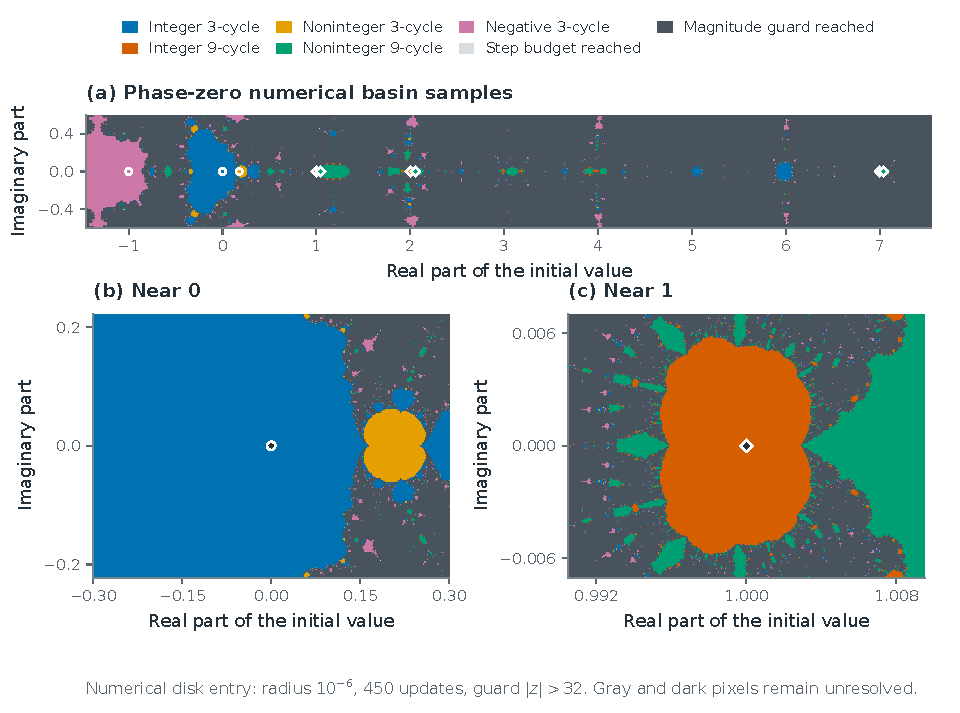
\includegraphics[width=.96\linewidth]{figures/complex_basins.pdf}
 \caption{Numerical basin views for the chosen cosine continuation
 at phase zero. The five target cycles have rigorous capture disks;
 the raster trajectories themselves are floating-point observations.
 Pixels reaching the magnitude guard or the iteration limit retain
 separate unresolved labels. Neither label proves divergence, and
 the five displayed attractors are not claimed exhaustive.}
 \label{fig:complex-basins}
\end{figure}

\FloatBarrier
\subsection{A real basin separator}

Put
$g(x)=R(x)-x$ for the return in \eqref{eq:complex-return}.

\begin{theorem}[Real separator]\label{thm:real-separator}
On $[0,9/50]$ the map $R$ is strictly increasing and has exactly
three fixed points: zero, a repeller
\[
 a\in(0.16503724,0.16503725),
\]
and an attractor
\[
 b\in(0.17752760,0.17752761).
\]
Every start in $[0,a)$ converges to zero under $R$, every start in
$(a,9/50]$ converges to $b$, and $a$ stays fixed. Moreover
$1.096<R'(a)<1.097$. The point $a$ lies on the boundary of both
corresponding open complex basins at phase zero.
\end{theorem}
\begin{proof}
The rational interval checker \path{certificates/geometry/separator.py}
covers the entire interval by closed subintervals and verifies
$R'>0$ on all of them. It verifies the following additional signs:
\begin{center}
\begin{tabular}{lll}\toprule
Interval&Strict sign&Number of certified subintervals\\\midrule
$[0,0.06]$&$g'<0$&6\\
$[0.06,0.15]$&$g<0$&5\\
$[0.15,0.17]$&$g'>0$&8\\
$[0.17,0.173]$&$g>0$&1\\
$[0.173,0.18]$&$g'<0$&4\\\bottomrule
\end{tabular}
\end{center}
At the two bracket endpoints for $a$, $g$ is respectively negative
and positive; at the two endpoints for $b$, it is respectively
positive and negative. Continuity and the strict monotonicity of
$g$ in those zones give exactly one zero in each bracket. Since
$g(0)=0$, the first two zones have no other zero. The remaining
strict signs exclude all other zeros in the interval. The derivative
enclosure on the first narrow bracket gives the repelling bound.
The second bracket is inside the independently certified capture
disk for the three-step noninteger orbit, identifying $b$ with that
orbit's phase-zero point.

The endpoint inequality $R(0.18)<0.18$ is checked directly, and
$R(0)=0$. Since $R$ is increasing, it preserves $[0,0.18]$ and an
iterate cannot cross a fixed point. For $0<x<a$, one has
$0<R(x)<x$; the decreasing orbit tends to a fixed point below $a$,
necessarily zero. For $a<x<b$, one has $x<R(x)<b$, so the orbit
increases to $b$. For $b<x\le0.18$, it decreases to $b$. Continuity
justifies the fixed-point property of each monotone limit.

The complex basins of zero and $b$ are open: each is a union of
preimages of an attracting neighborhood under continuous iterates
of $R$. Every complex neighborhood of $a$ contains real points
immediately to its left and right, belonging to these two different
basins. The repelling fixed point itself belongs to neither.
Consequently it is on both basin boundaries.
\end{proof}

The interval computation does not subtract two broad intervals to
estimate $g$ unnecessarily. On a box $[c-r,c+r]$ it encloses
$R'$ by the chain rule and uses
\[
 g([c-r,c+r])\subseteq g(c)+(R'([c-r,c+r])-1)[-r,r].
\]
For each physical step, the center value and derivative are bounded
by the same real Taylor method as above; the bound
$|C''|\le4+16(|c/2+1/4|+r/2)$ controls derivative variation on the
box. Every arithmetic interval is rounded outward to a rational
grid of denominator $10^{15}$. A failed strict comparison triggers
bisection, and an exhausted depth limit is an error. The saved leaf
intervals meet at their endpoints and cover each entire claimed
zone, so untested gaps cannot be hidden between sample points.

\begin{figure}[htbp]
 \centering
 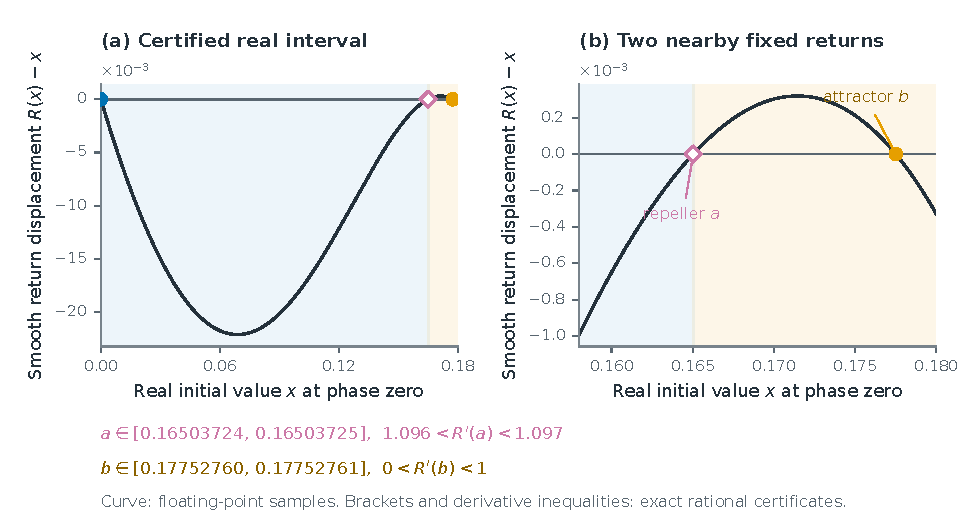
\includegraphics[width=.94\linewidth]{figures/real_separator.pdf}
 \caption{The phase-zero displacement $R(x)-x$ and the two nonzero
 root brackets. The curves are rendered numerically; the indicated
 signs, uniqueness of the three roots on $[0,0.18]$, and the basin
 partition are certified by the complete rational interval cover in
 Theorem~\ref{thm:real-separator}.}
 \label{fig:real-separator}
\end{figure}

\FloatBarrier
\subsection{The same complex point on three phase sheets}

Fix the complex starting point $w_*=71/100+\mathrm i/50$.

\begin{proposition}[Certified phase dependence]
\label{prop:complex-phase-dependence}
For the initial point $w_*$, launch phases zero and two converge
to the integer cycle $\Gamma_3$, whereas launch phase one converges
to $\Gamma_9$. The first entries into the radius-$10^{-6}$ disks
of the respective target cycles occur as follows:
\begin{center}
\begin{tabular}{rrrrl}\toprule
Launch phase&Updates&Arrival phase&Disk center&Destination\\\midrule
0&43&1&1&$\Gamma_3$\\
1&91&2&1&$\Gamma_9$\\
2&38&1&1&$\Gamma_3$\\\bottomrule
\end{tabular}
\end{center}
\end{proposition}
\begin{proof}
The checker \path{certificates/geometry/phase_trace.py} starts with
the radius-zero ball centered at the exact rational point $w_*$.
At every step it constructs a rational center $c_k$ and proves that
the true iterate lies in $|w-c_k|\le e_k$. Here is the error argument
that makes the finite calculation a certificate.

Reduce the real part of a center by its nearest integer and use
sine and cosine Taylor polynomials through degree 39 with rational
midpoint $\widehat\pi$. On the checked domain the reduced complex
argument has absolute value at most three. The tail is at most
$2\cdot3^{40}/40!$, by bounding successive exponential-series
terms geometrically. The uncertainty $\epsilon_\pi$ in $\pi$ adds
at most $8\epsilon_\pi$ to either trigonometric evaluation. The
constant eight follows from $|\operatorname{Im}w|<1/2$,
$\pi<4$, and the certified elementary bound $e^2<8$.
Write their combined bound as $\eta$.

The computed image polynomial is rounded to a rational center on a
$10^{-18}$ grid. Its rounding residual, together with
$|c_k/2+1/4|\eta$, bounds the error at the center. The analogous
derivative expression gives a rational upper bound $L_k$ on
$|C'(c_k)|$. Every enclosing disk satisfies
$|\operatorname{Im}w|<1/2$ and $|w|\le15$, on which
\eqref{eq:cosine-second} gives $|C''(w)|<2000$. Taylor's formula
along the segment inside the disk therefore permits the update
\begin{equation}\label{eq:complex-ball-error}
 e_{k+1}\ge \text{center residual}+L_ke_k+1000e_k^2.
\end{equation}
The checker rounds the right side upward to the $10^{-24}$ grid.
All remainder assumptions are verified again at every step; their
failure aborts the computation.

Let $r=10^{-6}$ and let $n$ range over the integer centers of the
target cycle on the current phase sheet. Before the claimed entry
time the checker verifies
$\min_n|c_k-n|^2>(r+e_k)^2$, excluding an earlier hit on those
disks. At the final time it verifies $e_k<r$ and
$\min_n|c_k-n|^2<(r-e_k)^2$, placing the entire error ball inside
a target disk. These are comparisons of rational numbers, without
square roots. The final errors are all less than $4\cdot10^{-18}$.
Proposition~\ref{prop:integer-capture-disks} then proves the
destinations in the table.
\end{proof}

All three terminal balls are near scalar height one. The first and
third are on phase one, where that integer belongs to $\Gamma_3$;
the second is on phase two, where it belongs to $\Gamma_9$.

\begin{figure}[htbp]
 \centering
 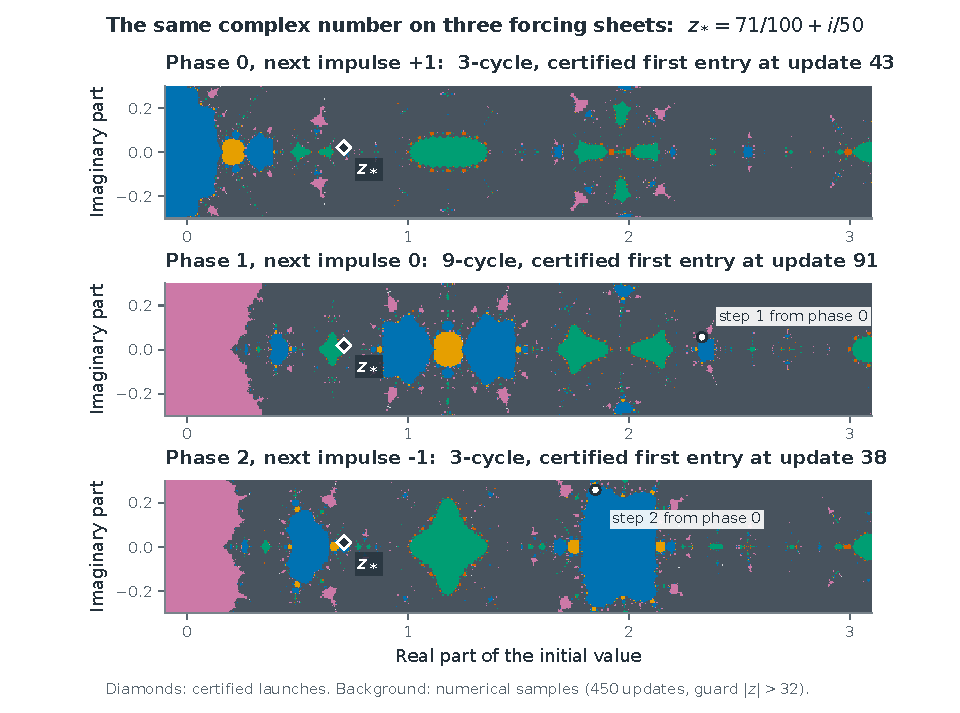
\includegraphics[width=.96\linewidth]{figures/phase_sheets.pdf}
 \caption{Three phase sheets of the same cosine continuation. Holding
 the complex coordinate fixed and changing sheets compares different
 launches; following a trajectory changes both its coordinate and its
 phase. The highlighted point $71/100+\mathrm i/50$ has the rigorously
 certified destinations and disk-entry times in
 Proposition~\ref{prop:complex-phase-dependence}. Background basin
 colors remain numerical samples.}
 \label{fig:phase-sheets}
\end{figure}

\subsection{Reproducing the geometry certificates}

Run
\begin{verbatim}
python3 -B certificates/geometry/verify.py
\end{verbatim}
with Python assertions enabled. The checker compares the eight integer
branches, three integer and two noninteger disk cycles, real interval
cover, and three complex-ball trajectories with
\path{certificates/geometry/certificate.json}. The figures sample a
finite grid. The total number of attractors remains open.

For the unforced cosine map, Lygeros and Rozier
\cite[Lemma~2.2]{lygeros-rozier-2014} provide a concrete link between
nearby real trajectories and integer orbits. With
$J_n^a=[n,n+a/(\pi^2n)]$, they prove
$C(J_n^a)\subseteq J_{T(n)}^a$ for all sufficiently large positive
integers $n$ when $27/8<a<6$, and for every positive $n$ when
$a=7/2$. A forced analogue would require intervals whose widths
depend on the phase. Translating the image by an impulse preserves
its width but changes the next center and denominator; those
inclusions and the small or zero centers would need new proofs.
